% checks commands
\RequirePackage[l2tabu, orthodox]{nag}

% document class
\documentclass[12pt, letterpaper]{article}

% language
\usepackage[english]{babel}

% bibliography
\usepackage{natbib}

% math
\usepackage{amsmath, amsthm, amssymb, commath, cool}

% add notes
\usepackage[colorinlistoftodos, textsize = scriptsize, color = yellow!90]{todonotes}
\setlength{\marginparwidth}{1in}

% spacing
\usepackage{setspace}
\onehalfspacing

% margins
\usepackage[letterpaper, margin=1.2in]{geometry}

% nice tables
\usepackage{booktabs}
\usepackage{ctable}
\usepackage{tabularx} 
\usepackage{subcaption}

% table columns
\newcolumntype{C}{>{\centering\arraybackslash}X}

% pictures
\usepackage{graphicx}
\usepackage[toc,page]{appendix} % make appendix
\usepackage[pdftex, unicode, pdfauthor={Olga Rud}]{hyperref}
\hypersetup{colorlinks, citecolor=blue, filecolor=black, linkcolor=blue, urlcolor=blue}
\graphicspath{{figures/}}

% theorems
\theoremstyle{plain}

% math operatores
\DeclareMathOperator*{\argmax}{arg\,max}
\DeclareMathOperator*{\mex}{\mathbb{E}}
\DeclareMathOperator*{\ind}{\mathbb{I}}
\DeclareMathOperator*{\prob}{\mathbb{P}}

% spacing in notes
\newcommand{\smalltodo}[2][]
     {\todo[caption={#2}, #1]
     {\begin{spacing}{1}#2\end{spacing}}}

\begin{document}

\newtheorem{Assumption}{Assumption}
\newtheorem{Proposition}{Proposition}
\newtheorem{Corollary}{Corollary}
\newtheorem{Hypothesis}{Hypothesis}
\newtheorem{Result}{Result}


\title{Timing in a conflict game: a laboratory experiment}

\author{Philip J. Grossman
\footnote{Department of Economics, Monash University} \and Youngseok Park\thanks{Korea Institute for International Economic Policy} \and Jean Paul Rabanal
\thanks{Department of Banking and Finance, Monash University (Corresponding author)}
 \and Olga A. Rud \footnote{Department of Economics, RMIT Univeristy} \and  \ }
\date{\today}
\maketitle


\begin{abstract}
We study how strategic commitment can enhance social welfare in a conflict game of incomplete information. We design gender balanced sessions to study whether gender differences affect convergence to the optimal solution. In the baseline treatment, players simultaneously commit to either a Hawkish, or Dovish action, where the latter can enhance social welfare. We add a sequential and an endogenous move treatment, where in the former, the first mover is exogenously selected and in the latter, players self-select the order of play. Our results suggest that (i) social welfare is higher in the last two treatments, and (ii) women prefer to guarantee a minimum payoff by playing Hawk when the order of play is endogenously determined.

\end{abstract}
\textbf{Keywords:}
gender; type uncertainty; endogenous timing; laboratory experiment\\
\textbf{JEL codes:} C72, C92, D82, D91
\newpage
\section{Introduction}
\label{sec:intro}
In certain conflict scenarios, precommitment to strategy can facilitate coordination and lead to Pareto superior outcomes. For example, consider a situation in which a bank run is possible. Agents are faced with the dilemma of whether to withdraw ($H$) or not ($D$) their savings from the bank. If agents have private idiosyncratic costs for $H$ (shoe leather costs), then it is cheaper for some agents to play $H$ than for others. However,  given that the game has strategic complementarity, the optimal strategy for the majority of agents is to follow the actions of other players, which can lead to two possible outcomes: (i) a bank run, where everyone plays $H$, or (ii) bank solvency, where everyone plays $D$. Precommitment to $D$ by some players can help avoid a bank run by motivating others to keep their savings in the bank. 

To study the role of precommitment in conflict games with strategic complements, we propose a laboratory experiment where we vary the timing of play.  We study three environments, characterized by incomplete information: (i) simultaneous (CGO), first proposed by Baliga and
Sj\"ostr\"om (2004, hereafter BS04), (ii) sequential (CGS), where the order of play is exogenously imposed, and (iii) endogenous (CGE), where players self-select the order of play (see Park and Rabanal, 2019). In the latter environment, when both players select to move first (second) the game becomes simultaneous and equivalent to CGO. When the players select different order of play, then the game becomes sequential and equivalent to CGS. Thus, the CGE treatment can resemble both the simultaneous and the sequential treatments, depending on the self-selected order of play. The CGE treatment is also characterized by strategic uncertainty, which arises from not knowing the action of the counterparty, nor the timing of play. 

Our experimental design adds two layers of novelty to related literature: (i) we elicit cutoff strategies across all treatments using a slider, which results in a rich distribution of choices across treatments, and (ii) we design gender balanced sessions to study whether gender differences affect convergence to the optimal solution. The experimental results show that players move their cutoff strategy according to theory, which means that they are willing to play $D$ more often in CGS treatment relative to the CGO treatment.

The results from the CGE treatment suggest that player strategy depends on whether the game is viewed as simultaneous or sequential. If a player chooses to move first and selects a cutoff similar to the one observed in CGO (CGS) environment, then the player is treating the game as simultaneous (sequential). Furthermore, in the CGE treatment gender appears to affect how the game is viewed by players ---as a CGO or a CGS. Our analysis of the CGE treatment shows that women prefer to (i) move first, and (ii) guarantee a minimum payoff by playing $H$, which means that they treat the CGE game as a CGO game. In fact, the cutoff chosen by women in the CGE treatment is similar to the one observed in CGO. Men respond differently than women to the CGE environment. They select a cutoff similar to the one observed in CGS, and have a preference for moving second where the initial strategy choice is non-binding. Therefore, the results of our study suggest that women prefer to have more control of the payoff distribution than men by imposing a definitive lower bound on earnings. Such behavior is also consistent with minimizing risk.

We do not find any statistical difference in the willingness to play $D$, the socially optimal strategy, across gender in the CGO and CGS treatments. Both men and women have the same distribution of cutoffs within each treatment. Thus, we can conclude that gender characteristics do not matter for achieving the social optimum in the CGO and CGS environments. Although the direction of the cutoff differences across CGO and CGS follows the theoretical predictions, both men and women fall short in selecting the Nash Equilibirum (NE) cutoff under the assumption of risk neutrality. This produces a lower joint frequency of $DD$ pairs in the CGS treatment compared to the theoretical prediction. In the CGO treatment, on the other hand, we observe that both men and women are willing to select a higher cutoff strategy relative to NE, which improves social welfare outcomes. 

\section{Related literature}

The present paper is related to the studies of Evdokimov and Garfagnini (2018), and Khan (2017) who also test the predictions of the CGO game first proposed by BS04, and observe higher frequencies of $DD$ play than predicted by NE. These studies do not use a cutoff strategy, which appeared in Duffy and Ochs (2012) and most recently in Van Huyck et al. (2018). The last authors survey participants about how they play the game and find that 72 percent report using a threshold. Similar to the behavior observed in our experiment, Duffy and Ochs (2012) also find that there is a significant variation in cutoff strategies across subjects. 

Strategic uncertainty, which exists in our CGE environment, can act as a barrier to superior outcomes and is common in coordination games (see Van Huyck, et al., 1990). CGS helps resolve this uncertainty, as shown by Weber et al. (2004) who find that it is sufficient for the subjects to know that game is sequential in order to improve welfare. Our work is also related to previous experiments which study cutoff strategies in games of incomplete information with strategic complements.\footnote{For a theoretical description of pre-commitment in games of complete information with strategic complements and/or substitutes, please refer to Eaton (2004).} Brindisi et al. (2014) find that, in an investment game with correlated player types (a joint investment opportunity), endogenous timing improves social welfare. The results indicate that while coordination is higher under endogenous timing, it is still lower than predicted. In the simultaneous-move game, subjects use a cutoff strategy which deviates from theory, and approaches payoff dominance--- similar to what we observe in our CGO treatment. Other games of incomplete information (Van Huyck et al., 2018) and complete information (Heinemann et al., 2004 and Duffy and Ochs, 2012) also report similar findings. However, for some classes of simultaneous-move games of incomplete information, risk dominance becomes an important factor in strategy selection (Cabrales et al., 2007).

According to the experimental results of Heggedal et al. (2018), risk aversion can deter a first mover from committing to an irreversible action. Their study tests the main predictions of Farrell and Saloner (1985), which is closely related to the environment of BS04. In stage one, players simultaneously decide whether to: (i) remain at status quo (known payoffs) or (ii) choose an alternative (risky payoff) which is irreversible. In stage two, only those players who have not yet committed to an action choose between the two alternatives. If no player committed to an action in stage one, then second stage decisions become simultaneous. The results show that, when the risk of failure is low, players are willing to commit and that they follow the equilibrium cutoff strategy. When the risk of failure is high (i.e. a large payoff loss if the other does not follow through) players are less willing to commit and the behavior deviates from the theoretical prediction. These findings are similar to what we observe in our CGS treatment and partially in our CGE treatment.

Lack of cooperation has also been observed in situations where women appear to be more averse to the ``sucker" effect, which occurs when individuals free-ride because they believe that others will as well (see Ingram and Berger, 1977; and Van den Assem et al., 2012). A recent lab-in-the-field experiment in rural India by Gangadharan et al. (2019) finds that women leaders contribute less than they propose in a public goods game, possibly supporting the notion that women fear being the ``sucker." However, according to Babcock et al. (2017) women can overcome the ``sucker" effect in a volunteer game with strategic substitutes. Their results show that women are willing to volunteer more often than men, although it may be costly. This suggests that when there is less payoff uncertainty, women may volunteer more and thus improve social welfare. However, in our game of strategic complements, resolving the payoff uncertainty by choosing $H$ does not lead to Pareto superior outcomes and in fact makes the CGE game resemble CGO. The preference for safe payoffs by women compared to men is also well documented in Crosetto and Filippin (2017).


\section{The conflict game}
\label{sec:model}
We model our environment after the simultaneous move two-player conflict game of BS04. In this game of incomplete information, player $i$ can pursue either a hawkish (aggressive) action ($H$), or a dovish (peaceful) action ($D$). The action space for a player can be specified as $s\in\{H,D\}$, and leads to the following payoff matrix
\begin{equation}
\begin{pmatrix}
x_i & \mu+x_i \\
k-d & k 
\label{t:payoff}
\end{pmatrix}.
\end{equation}
where $k=100$, $\mu=10$ and $d=95$. When both players play $H$, each player receives $x_i$, which is an idiosyncratic private payoff that is independently drawn from a uniform distribution $F\in [0,k]$. Therefore, the idiosyncratic $x_i$ can be thought of as hawk type, where some players are revealed to be more hawkish and thus reap more benefit from action $H$, and some are revealed to be less hawkish and see a lower return to playing $H$. If both players choose the peaceful action $D$, then the payoff to each player is a constant $k$. If player $i$ plays $D$, while player $j\neq i$ plays $H$, then the payoff to player $i$ is $k-d>0$, where $d$ can be considered a cost of a peaceful action when the opponent is aggressive. On the other hand, if player $i$ plays $H$ and player $j\neq i$ plays $D$, then the payoff to player $i$ is $\mu+x_i$, where $\mu (<d)>0$ can be viewed as a marginal benefit of an aggressive action when the opponent is peaceful. 

The Bayesian Nash Equilibrium (BNE) can be characterized as a cutoff strategy, following BS04, such that a player with a payout lower than $x_i\leq\hat{x}_{_{CGO}}$ will play $D$, and $H$ otherwise.  When a player is indifferent between $H$ and $D$, we can find the cutoff as the unique fixed point where 
\begin{equation}
\hat{x}_{_{CGO}}:= k-d + (d-\mu) F(\hat{x}_{_{CGO}}). \label{eq:cgo}
\end{equation}

\noindent Given that $F(\cdot)$ follows a uniform distribution in the space $[0,k]$, the cutoff point can be rewritten as 
\begin{equation}
\hat{x}_{_{CGO}}:= \frac{k\cdot (k-d)}{k-d+\mu}=33. \label{eq:cgosol}
\end{equation}
A possible mechanism for improving welfare in a CGO game is for players to move sequentially, in either an exogenous sequential move game (CGS) or/and an endogenous move game (CGE). In the former, the order of play is randomly determined while in the latter players self-select the order of play. Social welfare under a CGS game is significantly higher relative to the CGO game. However, in a CGE game social welfare can be similar to either the CGO or a CGS environment, depending on the order of play selected by players. We begin by describing the optimal strategy in a CGS game, where a player is randomly selected to move first. 

The cutoff strategy for the first mover in a CGS game shifts to the right of the optimal strategy in a CGO game, such that $\hat{x}_{_{CGO}}\leq\hat{x}_{_{CGS}}$. That is, in order to play $H$ in a CGS environment, a player has to be more hawkish, or requires a higher payoff to $H$. The intuition for the rightward shift in the cutoff strategy is fairly straightforward. Consider a first-mover at the original cutoff $\hat{x}_{_{CGO}}$. If the first-mover selects $D$, then she will obtain greater expected profits because the probability that the second mover will play $D$ as well is higher due to strategic complementarity. In other words, the probability that the other player plays $D$ increases from $Pr(x\leq\hat{x}_{_{CGO}}) \equiv F(\hat{x}_{_{CGO}}) $ in the CGO game to  $Pr(\mu+x_j\leq k) \equiv F(k-\mu)  $ in the CGS game. The unique Perfect Bayesian Nash Equilibrium (PBNE) where the first mover uses the cutoff strategy can then be defined as
\begin{equation}
\sigma_i(x_i)=D \quad \text{if} \ \ x_i\leq \hat{x}_{_{CGS}}:= k-\mu=90. 
\end{equation}

\noindent \textit{Proof:} See Appendix A $\blacksquare$

In the CGE game, where the players self-select the order of play, the timing of the game proceeds as follows:

\textit{Stage 0:} Each player $i$ selects a cutoff strategy, indicating a set of values where $\sigma_i(x_i)=H$, and then observes own type $x_i$, but not the other player's type $x_j$ where $j\neq i$.

 \textit{Stage 1:} Both players simultaneously select the period in which to play the game $t=1,2$. 

\textit{Stage 2:} The conflict game is played by the move structure determined in Stage 1. The commitment to the cutoff strategy is not binding for the player $i$ if and only if $t_i=2$ and $t_j=1$. 

The predictions for the CGE game follow the CGO and CGS solutions. Note that if both players select the same time period (e.g. $t=1$), then the environment resembles a simultaneous move game and the equilibrium follows the cutoff strategy specified in BS04. Therefore, in one possible equilibrium, $\hat{x}_{_{CGE}}=\hat{x}_{_{CGO}}=33$ and no player has incentive to deviate. Alternatively, players can coordinate and follow the strategy described in the CGS game, which leads to a different equilibrium where type $x\leq \hat{x}_{_{CGS}}\equiv 90$ will select $t=1$ and commit to $D$, while type $x>\hat{x}_{_{CGS}}$ will wait to play at $t=2$. Again, under this equilibrium players do not have any incentive to deviate. 

\noindent \textit{Proof:} See Appendix A $\blacksquare$
\\

\noindent \textbf{Prediction 1}
\textit{In the simultaneous conflict game (CGO) subjects play at or above the cutoff strategy $\hat{x}_{_{CGO}}=33$.}\\

We reconcile the theoretical solution in the CGO game with experimental evidence for our first prediction. In the laboratory, subjects play $D$ more often than predicted by the Nash Equilibrium (NE). \\

\noindent \textbf{Prediction 2}
\textit{The cutoff strategy in the sequential CGS game is higher compared to the cutoff strategy in the simultaneous move CGO game.}\\

Note that the equilibrium predictions $\hat{x}_{_{CGS}}=90$ and $\hat{x}_{_{CGO}}=33$ are far apart. This allows us to observe meaningful differences even when players chose cutoff values greater than the NE described in Prediction 1. The gain in expected payoff is equal to $d\times \left( F(\hat{x}_{_{CGS}})-F(\hat{x}_{_{CGO}}) \right)=95\times( 90-33)/100=50$ points or 137 percent. \\

\noindent \textbf{Prediction 3A} \textit{In CGE, a player will behave as in the CGO. }\\
\noindent \textbf{Prediction 3B} \textit{In CGE, a player will behave as CGS.}\\

The CGE environment can lead to multiple equilibria. At this point, we are uncertain about the type of equilibrium that would prevail in our experiment. Two conflicting Predictions, 3A and 3B, reflect our priors. \\

\noindent \textbf{Prediction 4}
\textit{The probability of observing a $DD$ outcome in either the CGS or the CGE game is greater than or equal to the probability of observing the same outcome in the CGO game.}\\

The coordination required to achieve the $DD$ outcome should be easier to achieve in a sequential game. Therefore, the frequency of $DD$ should be higher in the CGS game compared to the CGO game. The CGE game can lead to two outcomes, which depend on the selected order of play. If players choose the same order of play, then the CGE game should lead to the same outcome as predicted by the CGO game, where $\hat{x}_{_{CGO}}=33$ because the environment will resemble that of simultaneous play. However, if players select distinct time periods, such that $t_i\neq t_j$, then the game is sequential and the prediction becomes similar to one in the CGS environment.  Henceforth, we expect that the frequency of $DD$ under $\hat{x}_{_{CGE}}\geq \hat{x}_{_{CGO}}$.  \\

\noindent \textbf{Prediction 5}
\textit{There is no gender difference in strategy choices across the three games.}\\

As mentioned in the literature review, there are mixed evidence on the effect of gender in promoting social optimal outcomes. We do not take any strong position regarding the role of gender in all of our treatments. 


\section{Laboratory procedures}
\label{sec:game}

The experiment was conducted at the Rosario Experimental and Behavioral Economics Lab (REBEL) of the Universidad del Rosario, Colombia. Participants were undergraduate students from all fields and were recruited online via ORSEE (Greiner, 2015). Subjects were part of one of the three treatments (between design) ---CGO, CGS and CGE---  with  a session consisting of five practice periods and 11 paid periods. We pay the subjects for all periods because this is a game of incomplete information, where paying for only one period can increase the likelihood of hedging.\footnote{For the documentation in Spanish, language used in the sessions in Colombia, please contact the corresponding author.} Overall, we conducted nine sessions, with two silos per session. In each session there were two roughly gender-balanced silos of 12 subjects, each playing one of the three games. The participants were not informed that the study also focuses on analyzing possible gender differences.

\begin{center}
\begin{figure}[ht]
\centering{}%
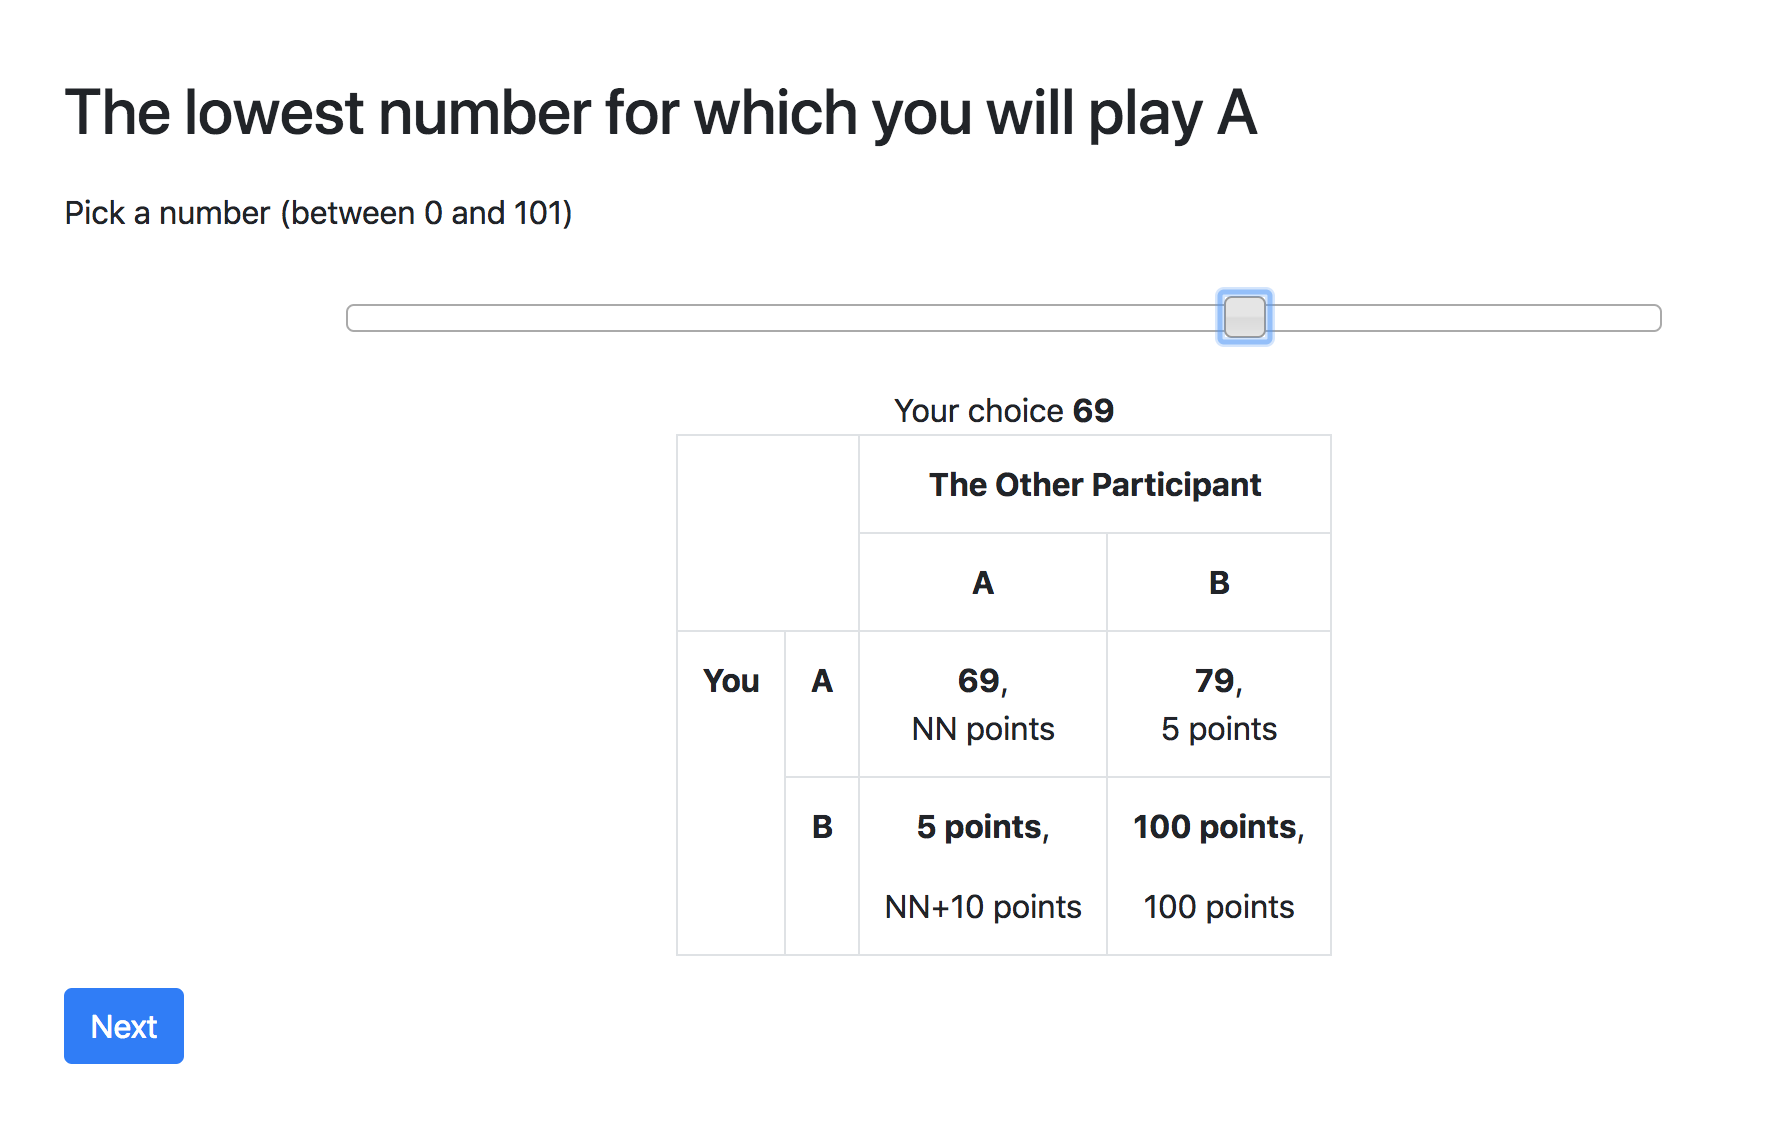
\includegraphics[scale=0.3]{cutoffen.png}%
\caption{User-Interface cutoff decision} 
\label{fig:ui}
\end{figure}
\end{center}
In each silo, the game began with five solo practice rounds, where the counterparty is a robot who plays the NE prediction.\footnote{The motivation behind using a robot initially is for subjects to learn how a threshold strategy works in our experiment.} The subject's task is to pick the minimum number of $x$ in the interval $[0,101]$ for which she will play $H$ (labelled $A$ in the experiment). That is, we directly ask the subject to select a cutoff strategy without having the knowledge of own $x$, and that of the counterparty. The user-interface designed in oTree (Chen, et al., 2016) is depicted in Figure \ref{fig:ui}. To select a cutoff value, the participant used the mouse to move the slider, and then confirmed her choice by clicking ``Next." For example, a subject who would like to play only $D$ ($H$) should move the slider to the extreme right (left). The user-interface in Figure \ref{fig:ui} presents the updated payoff matrix with the cutoff selection. In the payoff matrix, the unknown value of $x$ for the counterparty is depicted as $NN$.

Following the five practice rounds, subjects played 11 paid rounds. Each participant was matched with another participant only once (perfect stranger matching).  In all three treatments, subjects selected the cutoff simultaneously, and were unaware of the counterparty's gender. The steps following the cutoff selection varied according to treatment. We summarize the variations of the game in Table \ref{table:time}. 

\begin{table}[ht]
\begin{center}
\begin{tabular}{l|m{2.4cm}|m{3.5cm}|m{4cm}}
  Step & CGO & CGS & CGE\\
  \hline 
I & Cutoff & Cutoff & Cutoff \\
\hline
II& $x_i$ is revealed; H if $\mtext{cutoff}\leq x_i$ & $x_i$ is revealed; H if $\mtext{cutoff}\leq x_i$ for 1st mover (randomly chosen)
& $x_i$ is revealed; choose $t=\{1,2\}$ with action commitment defined according to $\mtext{cutoff}$\\
\hline
III & - & 2nd mover picks \textbf{s} & 2nd mover ($t=2$) picks \textbf{s} if other chose $t=1$. Otherwise, the game is simultaneous.

\end{tabular}
\end{center}
\caption{Timeline for each treatment}
\label{table:time}
\end{table}

In the CGO game, the value $x_i$ is revealed to player $i$. If the cutoff selected is smaller than or equal to revealed $x_i$ then the subject will play $H$, and $D$ otherwise. Following the actions, $H$ or $D$, of both players, payoffs are computed according to the payoff matrix in equation (\ref{t:payoff}). 

In the CGS game, the first mover is randomly selected after all subjects select the cutoff point. This ensures that the cutoff decisions are independent of the imposed order of play, and allows us to have a fairly balanced number of silos across treatments. It is also important to emphasize that the subjects know that the cutoff decisions are binding (relaxed) for first (second) movers. The second mover picks an action $s\in\{H,D\}$ conditional on the first mover's action. That is, the second mover does not face the same payoff matrix as presented to the first mover. Instead, the payoff matrix in the CGS game for the second mover reflects the action selected by the first mover, and is thus reduced to a matrix with dimension two by one. 

In the CGE game, after $x_i$ is revealed, subjects choose the order of play. If both players select the same period of play, then the game becomes simultaneous. If one player picks the first period while the other player picks the second period, then the game is sequential and the cutoff choice for the second mover is relaxed. The second mover makes a decision knowing the action of the first mover. 

\begin{table}[ht]
\centering
\caption{Sessions overview }
\hline
\begin{tabular}{lcccc}
  Treatment & Groups & Subjects per group & \% of women & Profit (mean, points)\\
  \hline  
  CGO & 6 & 12 & 51 & 701.6 \\
  CGS & 6 & 12 & 51 & 856.3 \\
  CGE & 6 & 12 & 47 & 820.7 \\
\hline
Total & 18 & 216 &  50 (mean) & 792.8 (mean)\\
\end{tabular}

\label{session}
\end{table}

At the end of each round, for all treatments, we provide feedback regarding own and counterparty choices, as well as individual payoff information. Following 11 rounds of play, accumulated points over all rounds were converted to COL at the exchange rate of COL 20 per point. Earnings, including a show-up fee of COL 10,000 (\$ 3.3), were paid in cash. On average, players earned 792.8 points (\$ 5.2) for a session that lasted under 45 minutes. Table \ref{session} presents the average profit as well as other relevant information per treatment. 


\section{Results}
\label{sec:results}

We begin by presenting in Figure \ref{fig:cutpooled} pooled data across all three treatments.\footnote{The data collected from the experimental sessions, as well as the data analysis included in this paper, can be found at \url{https://github.com/rabsjp/hdseq}.} 
\begin{center}
\begin{figure}[!ht]
\centering{}%
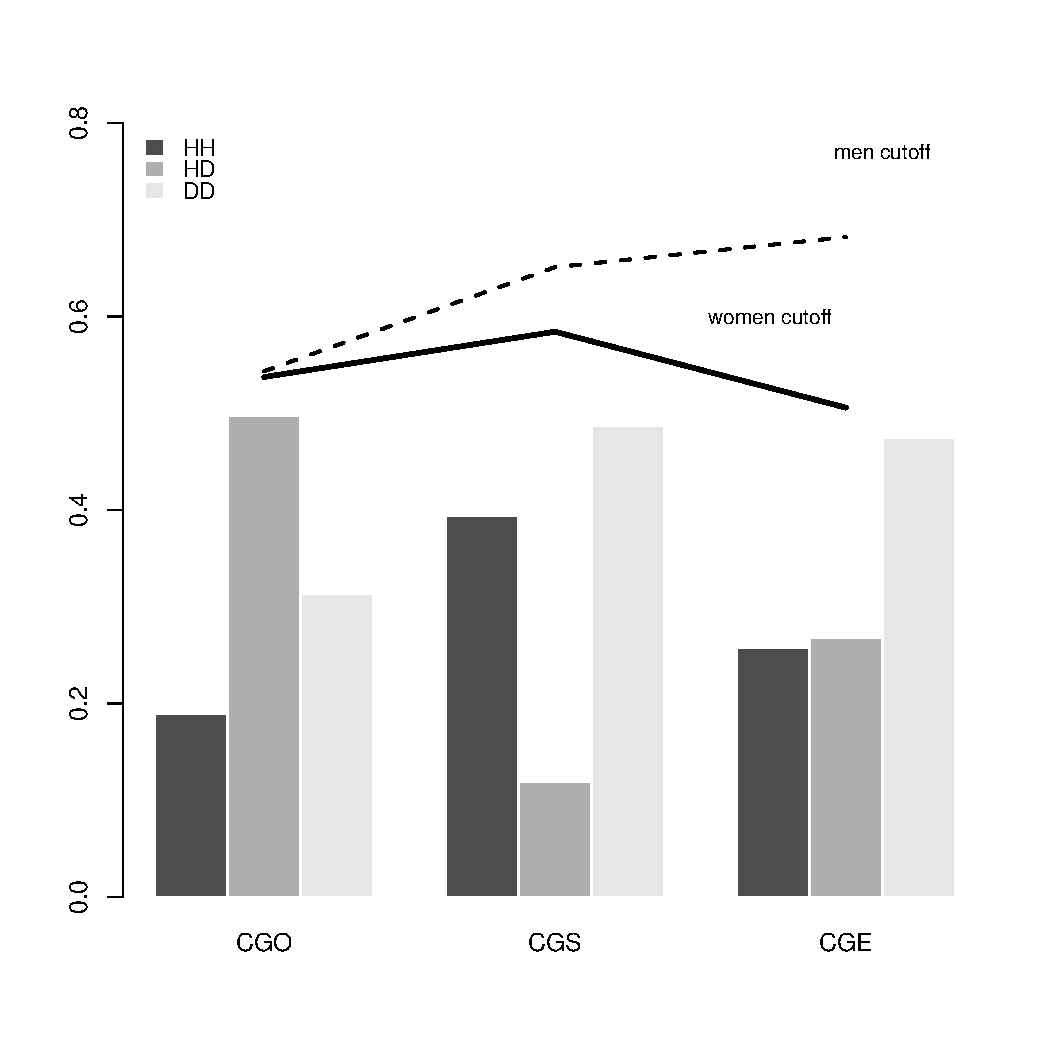
\includegraphics[scale=0.5]{jointcut.pdf}%
\caption{Cutoff strategy and cell relative frequencies across treatments (pooled data)} 
\label{fig:cutpooled}
\end{figure}
\end{center}
In the CGO treatment the mean cutoff is around 50 percent. We count the frequency of each outcome ($HH$, $HD (=DH)$ and $DD$) and determine that for the baseline CGO game (i) the $DD$ outcome is around 30 percent, and (ii) the off-diagonal cells appear most often, at around 50 percent. The outcomes for both the CGS and CGE treatments are quite different from the CGO outcomes. Subjects in the CGS game increase the mean cutoff value to around 60 percent, and men appear to increase the cutoff more relative to women. The sequential order of play helps achieve greater coordination with respect to $DD$ and $HH$ outcomes, which occur around 50 percent and 40 percent of the time, respectively. 




The CGE game presents a similar level of coordination with respect to the $DD$ outcome as the CGS game. The mean cutoff by gender, however, is quite different. The cutoff strategy chosen by women in the CGE game is similar to their strategy in the CGO game. The men, on the other hand, increase their cutoff strategy, relative to the CGS game. Next, we analyze gender differences in the CGE game according to strategy and order of play. The first two columns of Figure \ref{fig:cgepooled} present the time period $t\in\{1,2\}$ preference by gender. We can clearly see that men prefer to move second while women's choices are evenly distributed across both periods. Furthermore, men appear to play $D$ more often than women across both periods, which is consistent with the different cutoff strategies illustrated in Figure \ref{fig:cutpooled}.



\begin{center}
\begin{figure}[!ht]
\centering{}%
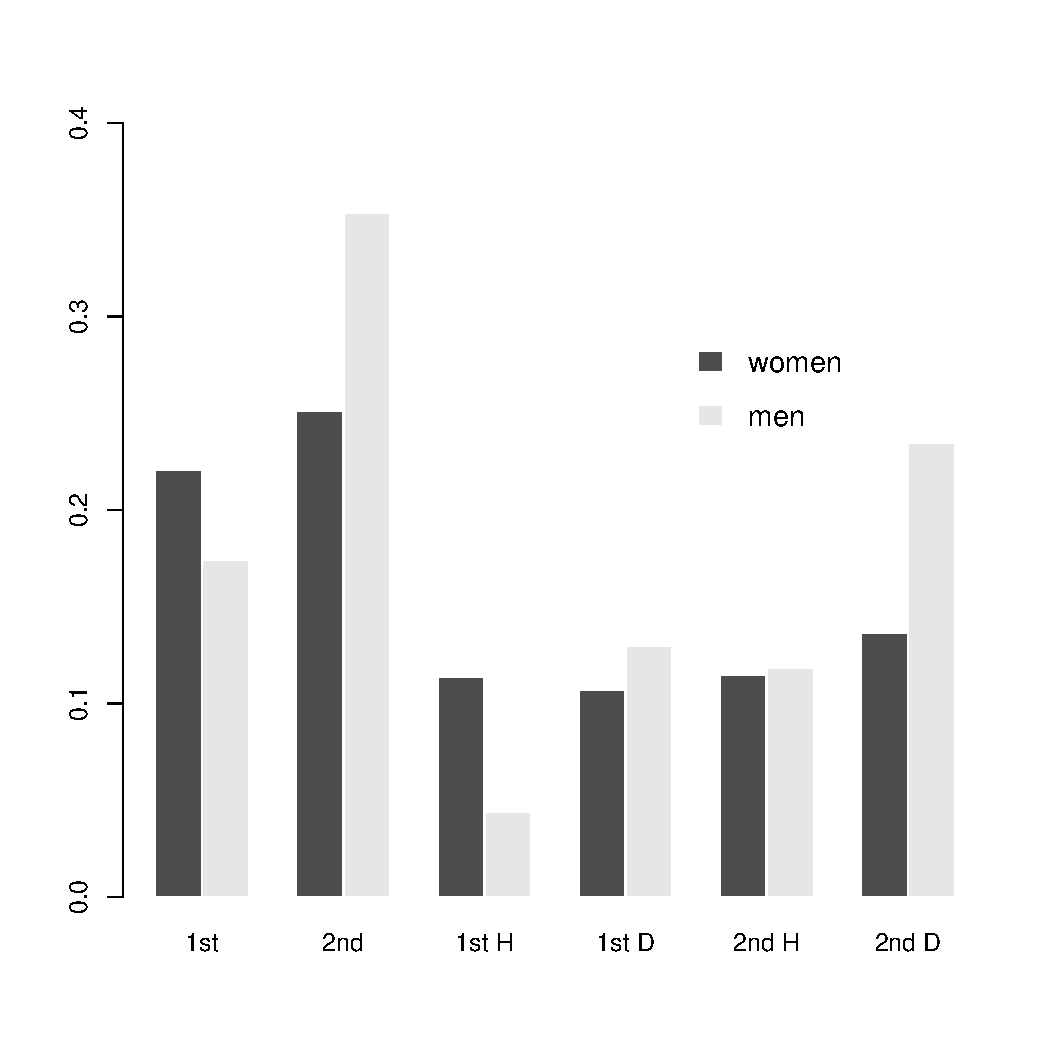
\includegraphics[scale=0.5]{countgendermoveplay.pdf}%
\caption{Strategy and order of play by gender (CGE)} 
\label{fig:cgepooled}
\end{figure}
\end{center}

Table \ref{tab(CGE)} details the frequency of the outcomes, $HH$, $HD(\equiv DH)$ and $DD$, tabulated according to the types of encounters possible in the CGE environment. That is, we summarize the frequency for each cell in a one-shot game played in the first period, one-shot game played in the second period, and a sequential order of play when subjects have different time preferences. About 52 percent of encounters occur sequentially. Of those, 56 percent lead to the $DD$ outcome. Most of the simultaneous encounters happen in the second period, and 41 percent of them lead to $DD$ outcome.  \\


\begin{table}[ht]
\centering\caption{Frequency (\%) by action and encounter type (CGE)}

\begin{tabular}{lccc}
\hline
 & One-shot 1st period & One-shot 2nd period  & Sequential\\
  \hline
  $HH$ &  2.27 & 5.56 & 17.93 \\
  $HD$ & 5.81 & 15.91 & 5.05 \\
  $DD$& 5.30 & 12.88 & 29.29 \\
  \hline
Total & 13.38 & 34.35 & 52.27\\
\end{tabular}

\label{tab(CGE)}
\end{table}

\begin{center}
\begin{figure}[!ht]
\centering{}%
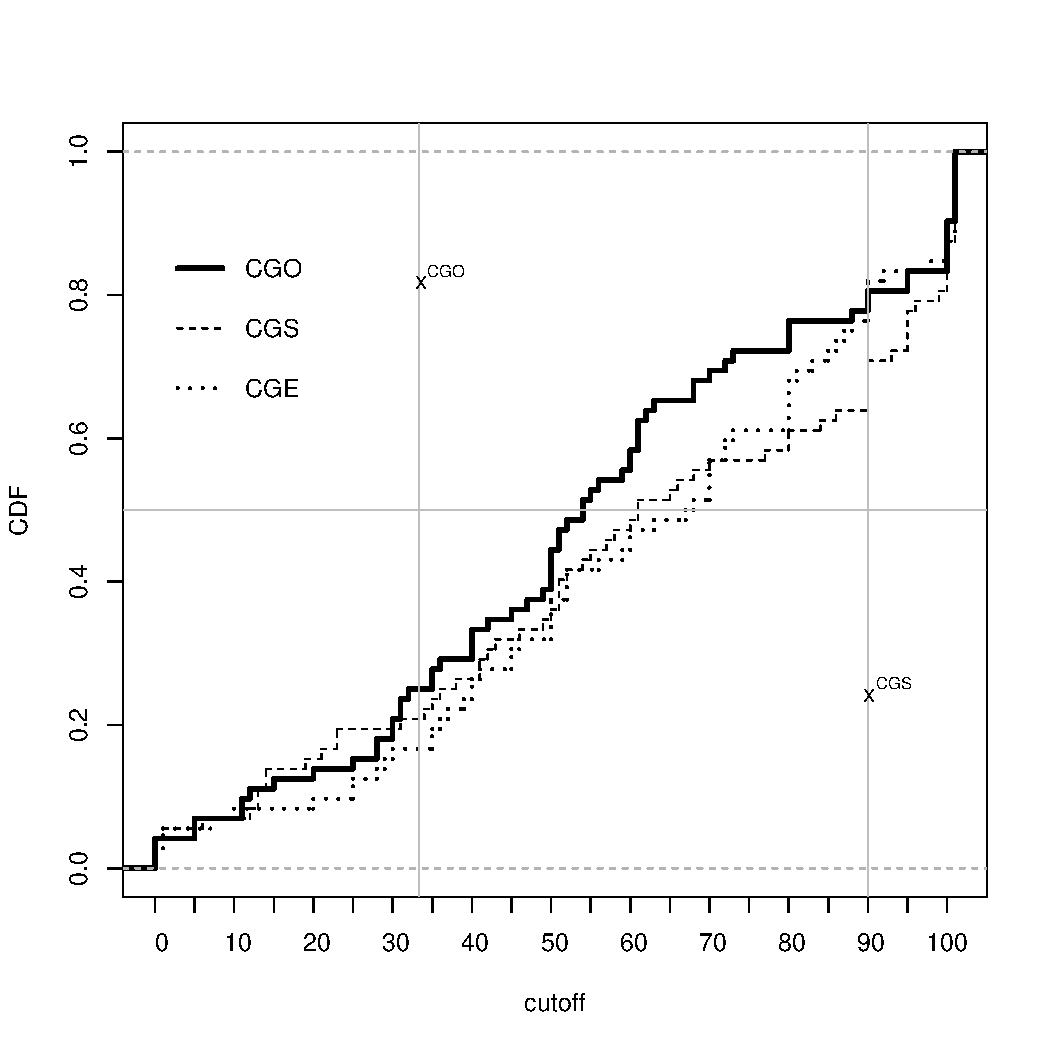
\includegraphics[scale=0.5]{cdfcutoff.pdf}%
\caption{CDF of cutoff strategies (subject data) \\ } 
\label{fig:allcutoff}
\floatfoot{\footnotesize{\textit{Note: $x^{CGO}$ ($x^{CGS}$) is the predicted cutoff in the CGO (CGS) game.}}}
\end{figure}
\par\end{center}


\noindent \textbf{Result 1}
\textit{The median cutoff strategy in the CGO game is 50 percent.}

We first take a conservative approach to testing our predictions. We compute the median cutoff chosen by each subject in rounds 6 through 11.\footnote{Regression analysis, shown further below, includes all 11 periods, with a trend variable to account for learning, confirms these results.} Figure \ref{fig:allcutoff} presents CDF by treatment. In the CGO game, we can see that the median value is around 50 percent, and that the distribution is fairly uniform, with some qualifications. About 20 percent of subjects pick the highest cutoff, which indicates that they strongly prefer to play $D$. Furthermore, we observe no significant mass centered around 33 percent, which is the NE prediction. In fact, the Kolmogorov-Smirnov (KS) test strongly rejects the hypothesis that cutoff strategy in the CGO game is equal to or below the NE prediction (the p-value is 2.2e-16).


To control for group effects we also perform panel regressions, presented in Table \ref{table:ols_all}, which confirm the results from our non-parametric analysis using all eleven periods. We evaluate three alternative dependent variables ---cutoff choice, profit and play of $D$---  on different regressors, including: variable CGS which takes on the value of one for the CGS treatment and zero otherwise; CGE which takes on the value of one for the CGE treatment and zero otherwise; the trend variable $Period$ which controls for learning throughout the session; the interaction between the trend and the treatments $Period \times CGS$ or $Period \times CGE$; the gender variable $Men$ which takes on the value of one when the subject is a man and zero otherwise; and the interaction effect between gender and treatments $Men \times CGS$ or $Men \times CGE$. The mean cutoff choice in the CGO treatment (specification I) is about 54 which is above the NE prediction of 33. Players get an average profit of 61 points (specification III).\footnote{The variable $Period$ is analyzed at the mean of six, when it is statistically significant.} Players in the CGO treatment decrease their cutoff choice in later periods as suggested by the negative sign of the trend, which weakly increases profit (the sign of the trend is positive in specification III, though not statistically significant). The extremely low $R^2$ in the regressions is due to the high heterogeneity observed in the cutoff choices (and therefore profit) common in these games (e.g. see Duffy and Ochs, 2012).\\

\begin{table}[ht]
\centering
\caption{Panel Regressions}
\footnotesize
\begin{tabular}{lccccc}

  & (I) & (II) & (III)  & (IV) & (V)\\
&  cutoff & cutoff  & profit & play D & play D \\
    \hline
Intercept & $57.83^{^{***}}$ &  $ 57.53^{^{***}}$ &  $61.03^{^{***}}$ & $.58^{^{***}}$& $.59^{^{***}}$\\
& (5.48) & (5.83)  & (4.94) & (0.04) & (0.06)\\
Period & $-.54^{^{***}}$ & $-.54^{^{***}}$  & $.26$ &  $ -.00$ & $ -.00$\\
& (.17)&  (.17) & (.48) & (.00) & (.00) \\
CGS & $-1.24$ &  $-4.22$  &  $14.82^{^{**}}$ &  $-.05$ & $-.08$\\
& (6.29) & (6.72) & (7.16) & (.09) & (.10)\\
CGE & $-3.47$ &  $-12.57^{^{*}}$   &  $3.43$ &  $-0.04$ & $-0.15^{^{**}}$\\
& (6.11) & (6.64)  & (5.95) & (0.07) & (0.06)\\
Period $\times$ CGS & $1.49^{^{***}}$& $ 1.49^{^{***}}$ & $-.15$ & .01 & .01 \\
& (.52) & (.49) & (.70) & (.01) & (.01) \\
Period $\times$ CGE & $1.56^{^{***}}$& $1.56^{^{***}}$ &$.85^{^{*}}$ & $.02^{^{***}}$ & $.02^{^{***}}$ \\
& (.36) & (.35)  & (.51) & (.00) &  (.00)\\
Men & --- &  $.61$ & .61  & $-.02$ &  $-.02$ \\
&  & (3.99) & (3.99)  & (.04) & (.04)\\
Men $\times$ CGS & ---&  6.13 &  .27 & --- & .07\\
& & (8.59) & (8.29)&  & (.08)\\
Men $\times$ CGE & ---& $17.20^{^{**}}$ & 4.31 & --- & $.19{^{***}}$\\
& & (6.06)& (8.20)&& (.06)\\

\hline
N & 2,376 & 2,376 & 2,376 & 2,376  & 2,376  \\ 
$R^2$ & 0.02 & 0.04  & 0.03 & 0.01 & 0.02\\
\hline
\hline
 \multicolumn{6}{p{.65\textwidth}}{\scriptsize{The dependent variable in (I) and (II) is the cutoff choice. In specifications (III) the dependent variable is the profit earned. (IV)-(V) is whether the subject play D(=1) or H(=0). Standard errors are in parenthesis, clustered at the group level and are computed via bootstrapping. Random effects are included at the subject level. }}\\ 
 \multicolumn{4}{p{0.4\textwidth}}{\scriptsize{ $^{^{***}}p\leq.01$,
    $^{^{**}}p\leq.05$, $^{^{*}}p\leq.1$}} \\
\end{tabular}
\label{table:ols_all}
\end{table}

\noindent \textbf{Result 2}
\textit{In the CGS game, players increase the median cutoff to 66 percent.}

The CDF for the CGS game first-order stochastically dominates the CDF for CGO game (the p-value of a Kolmogorov-Smirnov test for which the null states that $\hat{x}_{_{CGO}} \geq \hat{x}_{_{CGS}}$ is .006). The mass in the CGS game approaches the predicted NE of 90 percent, thought it still falls short. The median cutoff strategy is 66 percent. Similar to the CGO environment, some players in the CGS game also select either extremely high or extremely low cutoff values. Overall, the majority of players in the CGS game select a higher threshold relative to the CGO game, thus improving social welfare.\footnote{If we include all periods in KS test, we obtain a p-value of .19. Therefore, we fail to reject that CGO and CGS distributions are equal. The significance (at five percent) of the results appears from periods 3 to 11. Our sample includes periods 6 to 11 to account for learning.}

Table \ref{table:ols_all} compares the choices (specification I) and profit (specification III) in CGO and CGS treatments using panel regressions (OLS). The mean cutoff choice in the CGO treatment is lower than in the CGS treatment by about nine points. The average profit for players in the CGS treatment is higher by about 15 points. The interaction between the trend variable and CGS shows that players in the CGS treatment increase their cutoff strategy as the game progresses, contrary to the behavior observed in the CGO treatment. Thus, our results suggest that strategies are influenced by the environment, even though on average we observe similar frequencies of $D$ play (specification IV, Table \ref{table:ols_all}). The lack of statistical significance for the treatment variable in specification IV can be explained by the small number of observations we have to account for meaningful difference of play given that cutoff choices vary by approximately ten percent across treatments, and the choices are quite dispersed across subjects. In terms of profit (specification III), players in the CGS treatment perform about 15 points better than in CGO treatment. \\ 


\noindent \textbf{Result 3}
\textit{In the CGE game the median cutoff strategy is 70 percent.}

While roughly 25 percent of players select a low cutoff strategy similar to the one in the CGO game, the majority of players select a cutoff value such that $\hat{x}_{_{CGE}}> \hat{x}_{_{CGO}}$. There is also a sizable mass (35 percent) of players who select a cutoff strategy with values above the predicted NE of 90 in the CGS game. The overall distribution of cutoff strategies in the CGE game is quite similar to the one in the CGS game. We fail to reject the hypothesis that the two cutoff strategies come from the same distribution (KS test p-value of .77).

The regressions (see Table \ref{table:ols_all}) confirm that cutoff strategy (specification I-II) and play of $D$ (specification IV-V) are similar across the CGE and CGS treatment. We perform a Wald test in specification (I) and we fail to reject that interaction of period with the treatment variable CGS is equal to the interaction with  the treatment variable CGE. In terms of profit (specification III), players in the CGE perform slightly better than in the CGO (about 5 point difference).\\

\begin{table}[!t]
\centering
\caption{Frequency (percentage) of cell $DD$ played in groups }
\begin{tabular}{lccccccc}
\hline
Treatment & Group 1 & G2  & G3 & G4 & G5 & G6 & Mean\\
  \hline
  CGO &  19.44 & 19.44&  27.78 & 27.78 & 36.11 & 52.78 & 30.56 \\
  CGS & 30.56 & 47.22&  50.00 & 52.78 & 55.56 & 61.11 & 49.53\\
  GGE & 33.44 & 38.49 & 44.44 & 58.55 & 63.89 & 69.44 & 51.39 \\
  \hline

\end{tabular}

\label{table:dd}
\end{table}

\noindent \textbf{Result 4}
\textit{The $DD$ outcome appears more often in CGS and CGE environments.}

We compute the frequency with which $DD$ appears in each of the groups (of twelve people). Table \ref{table:dd} presents the sorted data and the mean per treatment. $DD$ occurs less often in the CGO environment across all six independent groups. CGS and CGE do not exhibit low $DD$ frequency ($<$ 30 percent), which appear in two-thirds of the CGO groups. More formally, non-parametric tests reject the hypothesis that the frequency of $DD$ in the CGO environment is greater than or equal to either the frequency of $DD$ in CGS (KS p-value of .069 and Wilcoxon p-value of .018) or CGE (KS p-value of .069 and Wilcoxon p-value of .015) environment. Additionally, we fail to reject the hypothesis that CGS and CGE come from the same distribution (p-value of a Wilcoxon two-sided test is 1.0).\footnote{We omit panel regressions when analyzing the joint frequency given that the non-parametric tests are at the group level which strictly satisfies the independence assumption across observations. Using all periods does not change the conclusions of our tests. When comparing CGO vs CGS, the KS test p-value is .016 and Wilcoxon test p-value is .020. When comparing CGO vs CGE, the KS test p-value is .069 and Wilcoxon test p-value is .063. }\\

\begin{center}
\begin{figure}[ht]
\centering{}%
\begin{minipage}[t]{0.45\columnwidth}%
\subfloat{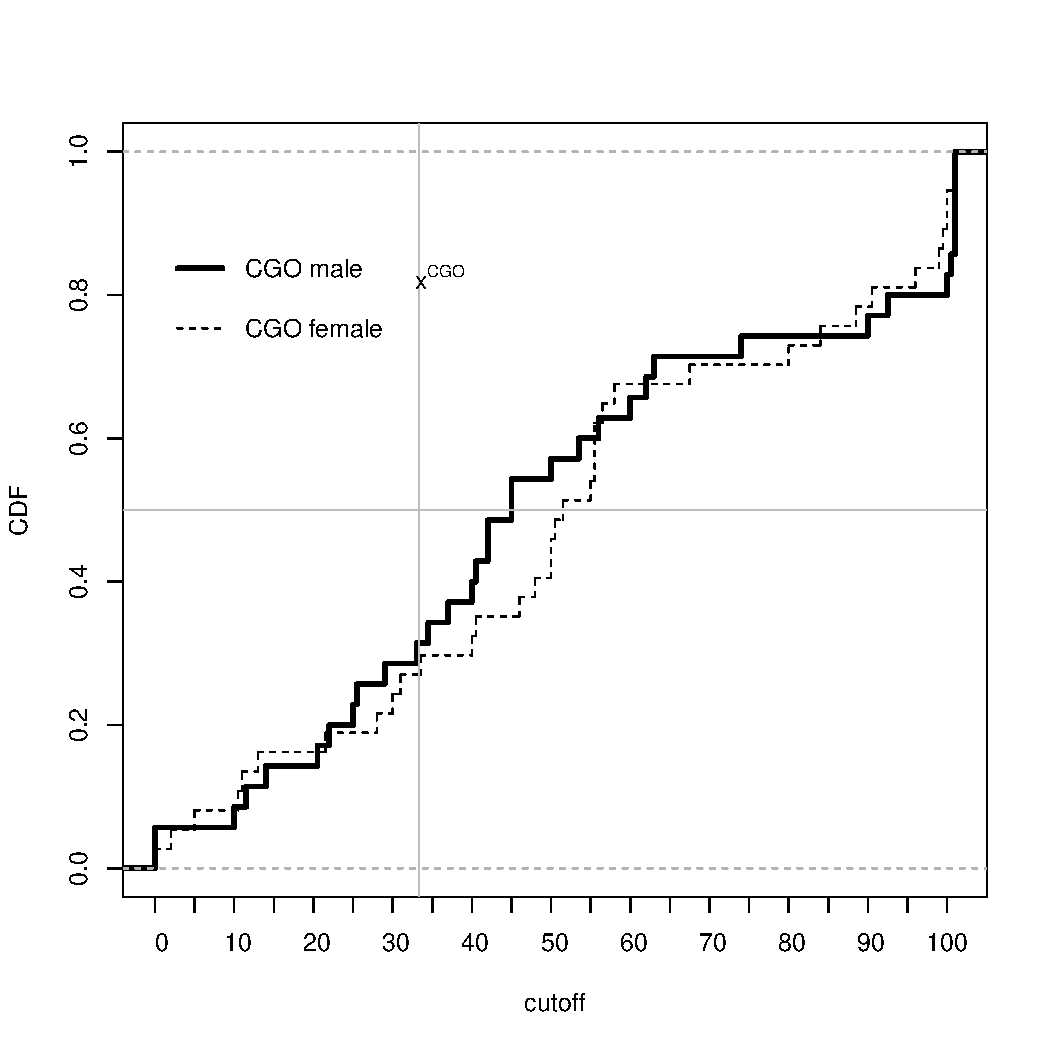
\includegraphics[scale=0.4]{cdfcutoffgender_o.pdf}}%
\end{minipage}%
\begin{minipage}[t]{0.45\columnwidth}%
\subfloat{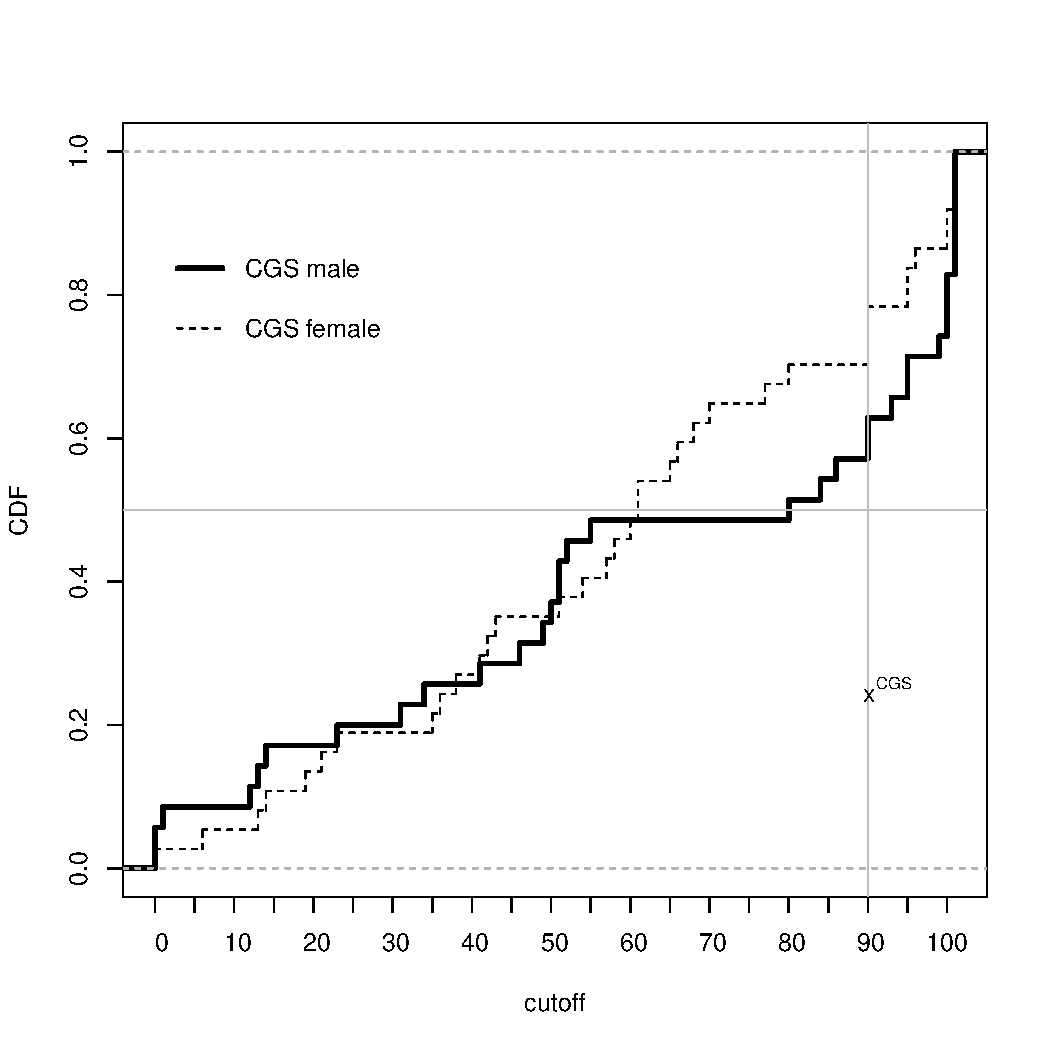
\includegraphics[scale=0.4]{cdfcutoffgender_s.pdf}}%
\end{minipage} 
%\captionsetup{font=large}
\caption{CDF of cutoff strategy choices in CGO (left) and CGS (right), by gender \\\footnotesize{\textit{Note: $x^{CGO}$ ($x^{CGS}$) is the predicted cutoff in the CGO (CGS) game.}} }
\label{fig:cdfgender1}\end{figure}
\par\end{center}

\noindent \textbf{Result 5}
\textit{Gender differences appear only in the CGE game. Men significantly increase their cutoff value, improving the frequency with which $D$ is selected, while women revert to a strategy similar to the one in the CGO game.}

We next analyze the cutoff strategy across gender. Figure \ref{fig:cdfgender1} presents the CDF of the cutoff strategy by gender in the CGO game (left panel) and the CGS  game (right panel). We find no difference in strategy in the CGO game (KS test p-value .52). In the CGS game, we observe a larger mass of men with a cutoff strategy that is greater than the predicted NE (90). The rest of the distribution looks quite similar across gender. In fact, we fail to reject the hypothesis that the cutoff distributions are equal in the CGS game (KS p-value of .54). It is important to note that in the CGS game, conditional on observing $D$ in the first period, we do not observe any gender difference among the second mover responses. There are about ten percent of women and men who follow $D$ with an $H$ choice, which is consistent with theory.

However, important differences emerge under endogenous timing. The cutoff strategy choices by men first order stochastically dominate the cutoff strategy choices by women, which we depict in the left panel of Figure \ref{fig:cdfgender2}. We reject the null hypothesis which states that men choose a cutoff strategy that is equal to or smaller than the one chosen by women, with a p-value of .001 for Wilcoxon and .006 for KS.\footnote{Using all periods, we also confirm the separation between cutoffs. The p-values are .06 for Wilcoxon and .01 for KS.} The cutoff strategy distribution for women in the CGE game resembles the one observed in CGO game. The cutoff strategy distribution for men shifts significantly to the right, such that the median value is closer to the one observed in the CGS game. The mass around the high cutoff strategy choices ($>$90) in both CGS and CGE is about 40 percent for men. This is quite different than the behavior observed in CGO, where the mass is about 20 percent. 

\begin{center}
\begin{figure}[ht]
\centering{}%
\begin{minipage}[t]{0.45\columnwidth}%
\subfloat{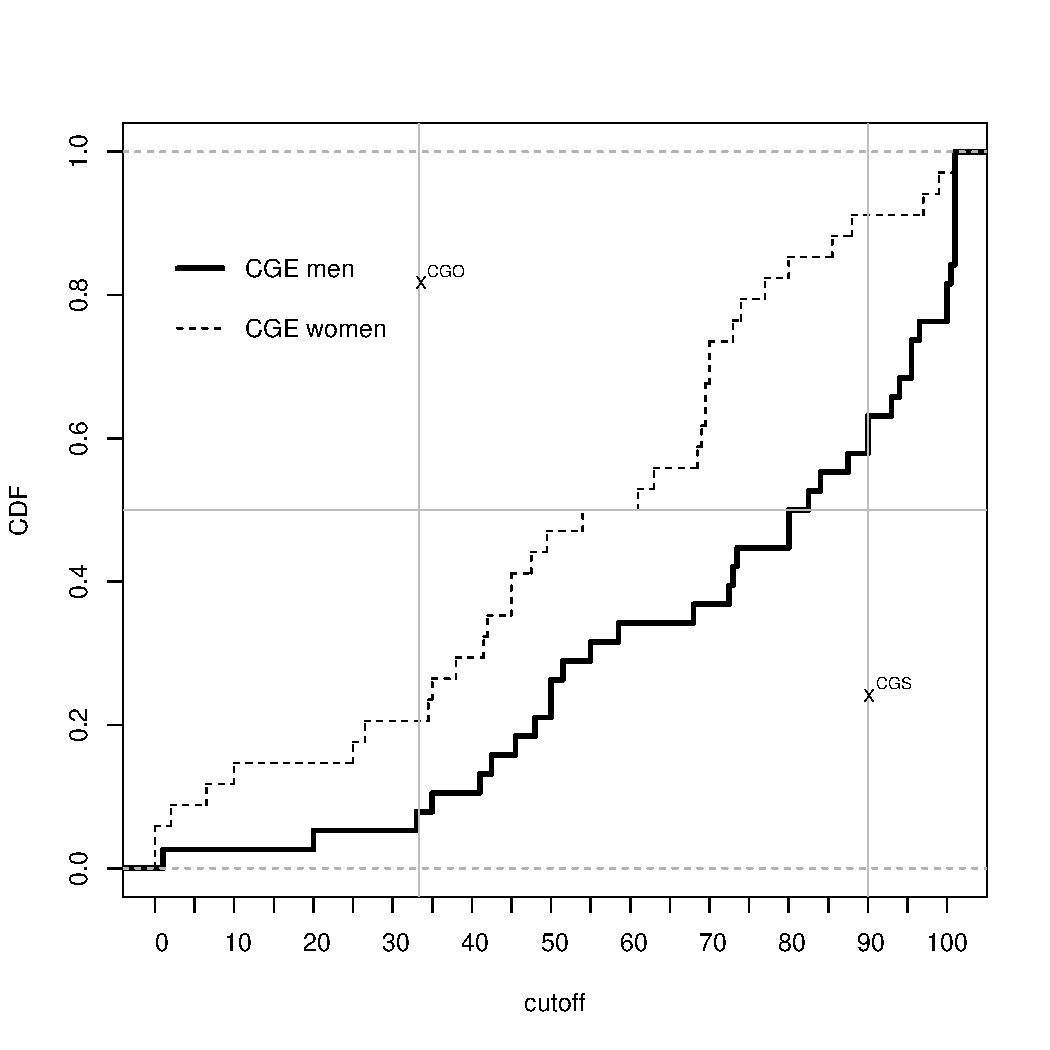
\includegraphics[scale=0.4]{cdfcutoffgender_e1.pdf}}%
\end{minipage}%
\begin{minipage}[t]{0.45\columnwidth}%
\subfloat{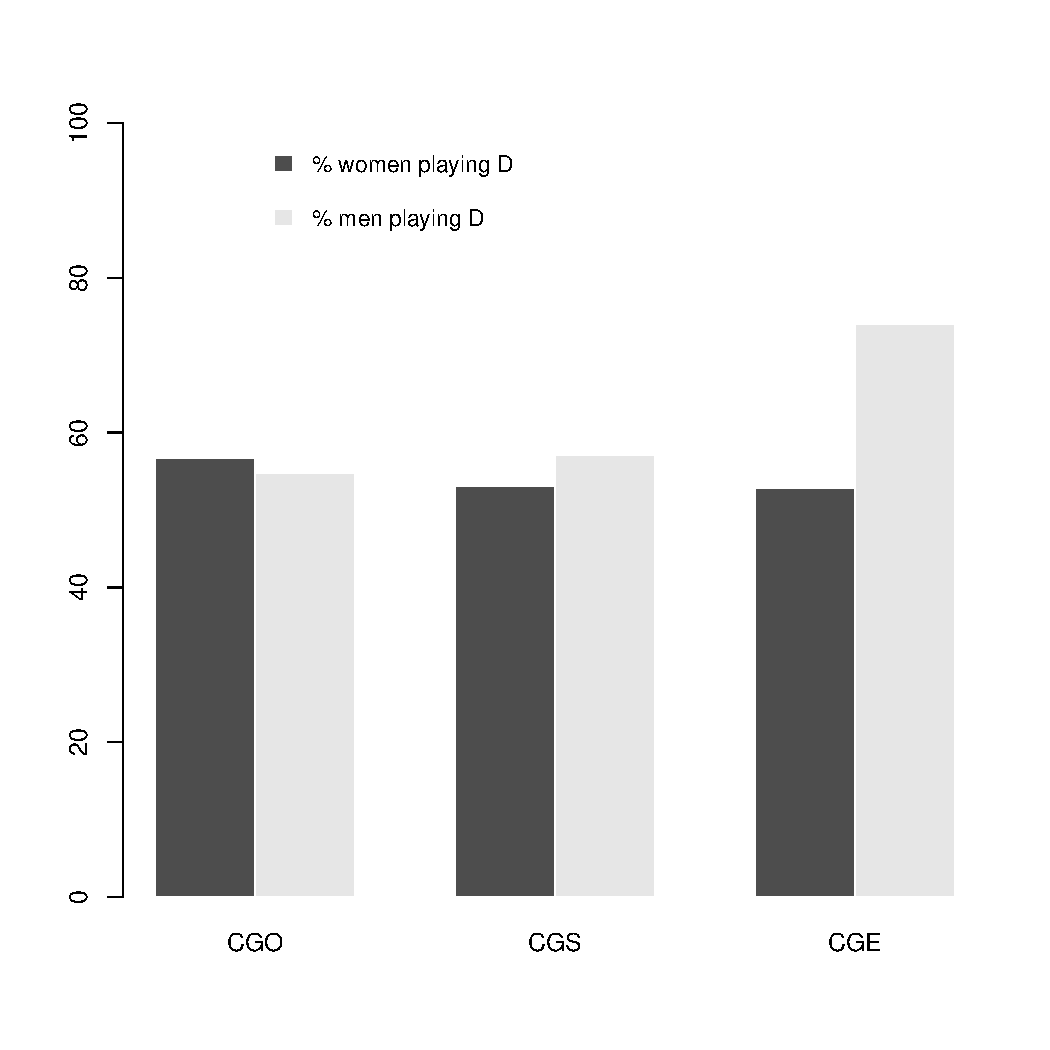
\includegraphics[scale=0.4]{genderplay1.pdf}}%
\end{minipage} 
%\captionsetup{font=large}
\caption{CDF of cutoff strategies in CGE (left panel) and $D$ play (right panel) by gender\\ \footnotesize{\textit{Note: $x^{CGO}$ ($x^{CGS}$) is the predicted cutoff in the CGO (CGS) game.}}}
\label{fig:cdfgender2}\end{figure}
\par\end{center}




The high cutoff values chosen by men translates to a higher frequency of $D$ play as shown in the right panel of Figure \ref{fig:cdfgender2}. Corroborating our earlier conclusion, the frequency of $D$ choices across gender shows neither statistical nor economic differences across CGO and CGS games. We find a difference in $D$ play across gender only in the CGE game. Specifically, in this environment the results show that men play $D$ at a rate of 20 percentage points higher than women. 

Table \ref{table:ols_all} also shows gender differences using panel (OLS) regressions. According to specification (II), the variable $Men$ is significant only in the CGE treatment. Women use a cutoff similar to the CGO treatment ($1.56\times 6-12.57= -3.21$) while men increase increase their cutoff relative to women by 17 points, which translates to a higher frequency of $D$ (19 percentage points, in specification V).
\begin{center}
\begin{figure}[ht]
\centering{}%
\begin{minipage}[t]{0.45\columnwidth}%
\subfloat{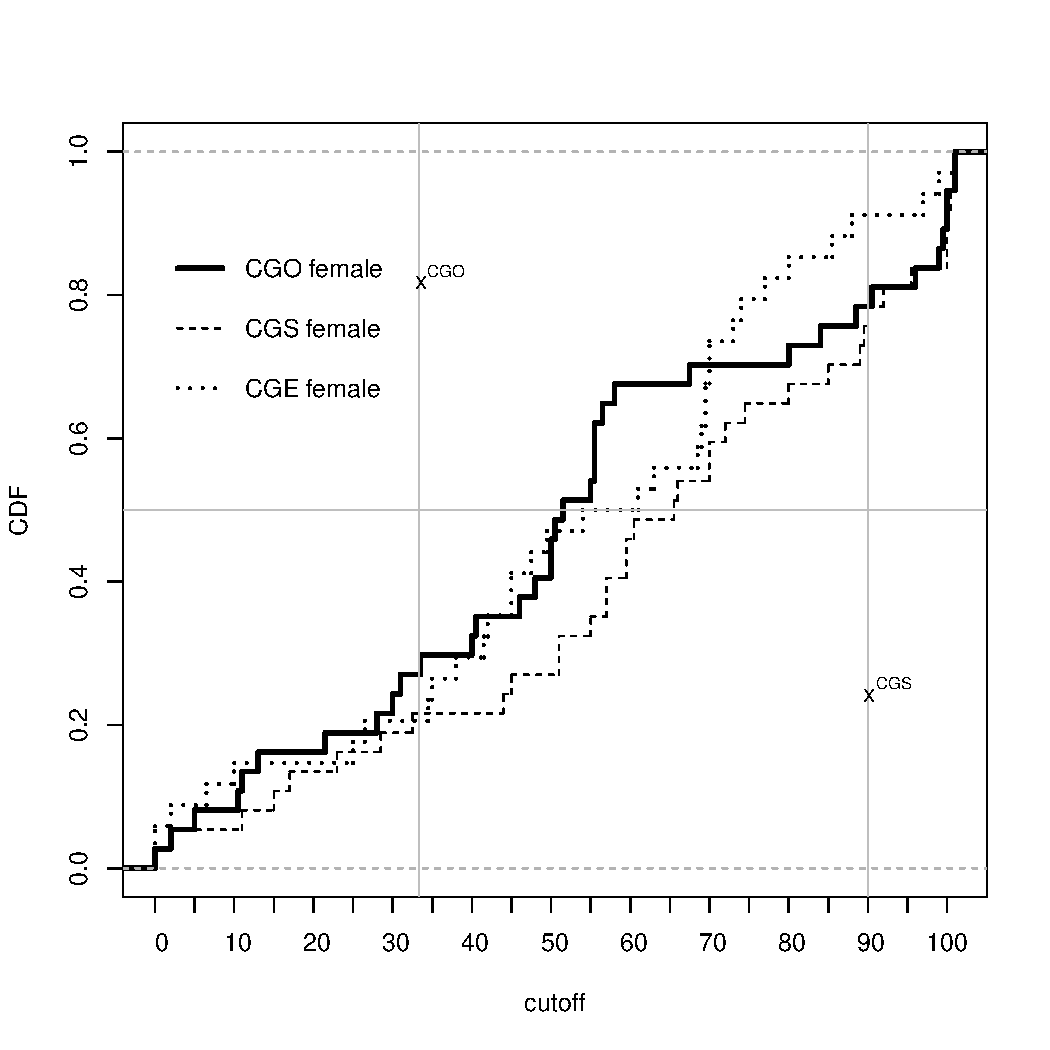
\includegraphics[scale=0.4]{cdfcutoffgender_female.pdf}}%
\end{minipage}%
\begin{minipage}[t]{0.45\columnwidth}%
\subfloat{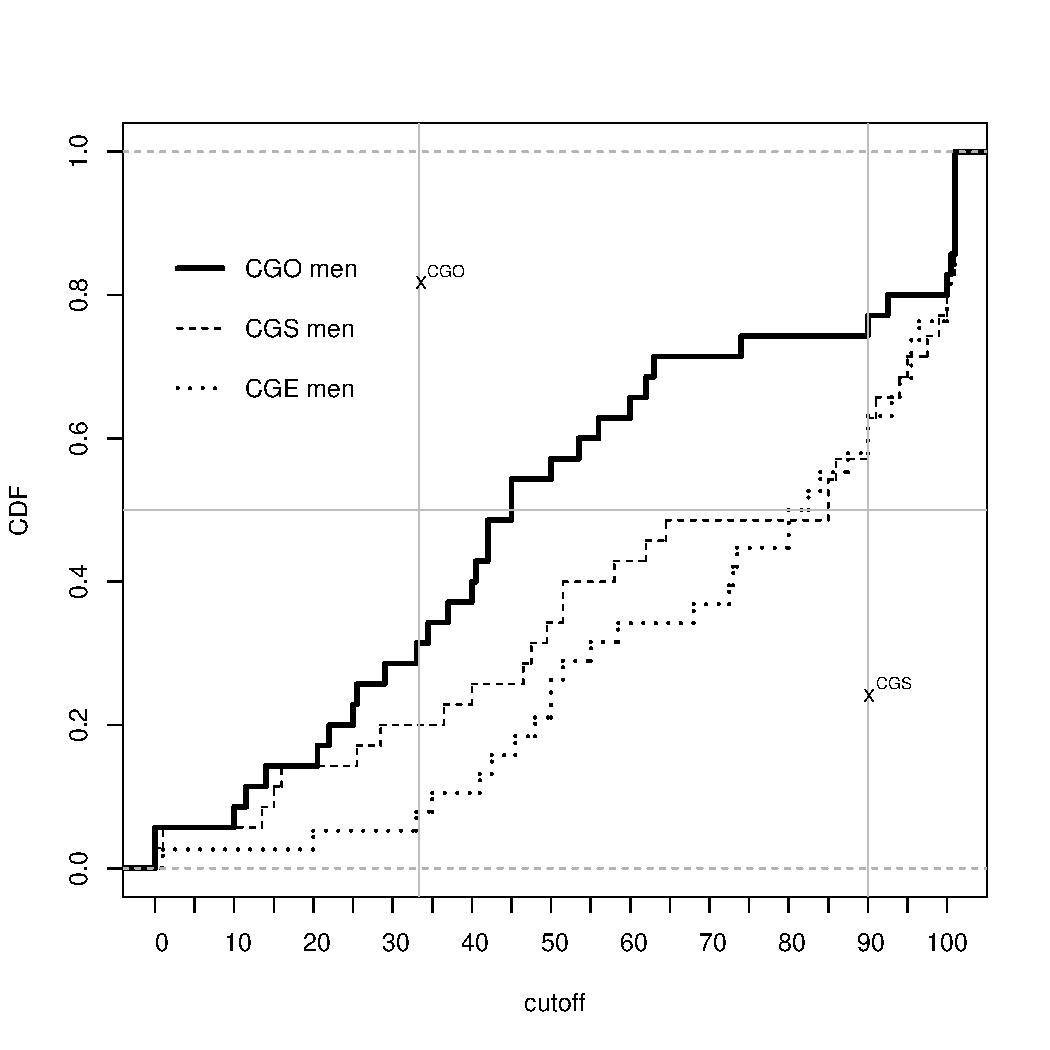
\includegraphics[scale=0.4]{cdfcutoffgender_male.pdf}}%
\end{minipage} 
%\captionsetup{font=large}
\caption{CDF of cutoff strategies for women (left) and men (right) across treatments\\\footnotesize{\textit{Note: $x^{CGO}$ ($x^{CGS}$) is the predicted cutoff in the CGO (CGS) game.}}}
\label{fig:cdfall}\end{figure}
\par\end{center}

\section{Discussion}
\label{sec:discuss}

In this paper, we provide experimental evidence on how strategic commitment can enhance social welfare in conflict scenarios. The experimental design includes (i) a simultaneous game, (ii) a sequential order of play, and (ii) an endogenous order of play. Furthermore, we seek to study whether gender differences are important to explain strategic behavior in conflict games of incomplete information. The results show that sequential order of play improves welfare relative to the simultaneous game. Gender is not important in explaining behavior of either game. When players are allowed to self-select the order of play, we find that women prefer to move first and adopt a cutoff similar to the one in the simultaneous-move game, meanwhile men prefer to move second and adopt a cutoff similar to the one in the sequential game. This suggests that the possibility of a first-period player selecting $H$ deters men from moving first, which requires precommitment since the strategy selection for the first mover is binding. 

Our results provide important insights to a variety of games of incomplete information. First, the strategic interaction of players is similar across gender when the underlying game is of strategic complements and therefore, one should not be surprised if gender differences are not observed. Second, there is a large heterogeneity in choices within each gender. Using a slider to implement cutoffs, we are able to observe the values which trigger Hawkish play. Third, risk attitudes across gender in endogenous move games are important in explaining behavior. Men prefer to wait and see what the first mover selects, while women prefer to guarantee a relatively safe payoff by moving first.  

Although we began by describing the BS04 game as a possible bank-run model, the game can be applied to other conflict scenarios such as negotiations of sanctions, or corporate disputes, where actions are characterized as strategic complements. For an overview of the experimental literature on conflict and contest games, please refer to Kimbrough et al., 2017. Future research can provide additional insights on the role of gender in other endogenous timing games. Our work is the first to encounter such differences in this class of games, and therefore further analysis is needed.  


\section{Acknowledgements}
We are grateful for the comments received from Lata Gangadharan, Marie Claire Villeval, Erte Xiao, Dan Friedman, Tomas Sj\"ostr\"om, Dann Arce, Nisvan Erkal, Diego Aycinena, Kyung Hwan Baik, Tim Cason, Tom Wilkening, Roman Sheremeta, Maria Recalde, John Duffy, Jin Yeub Kim, and seminar participants in numerous seminars and conferences. This research was supported by funds granted by Colby College. This project was approved by the IRB at Colby College and Universidad del Rosario.

\newpage
\begin{thebibliography}{10}

%\bibitem{} Andreoni, J., 1998. Toward a theory of charitable fund-raising. \textit{Journal of Political Economy,} 106(6), pp.1186-1213.

%\bibitem{} Avoyan, A., 2019. Communication in global games: theory and experiment. 

%\bibitem{} Azmat, G., Calsamiglia, C. and Iriberri, N., 2016. Gender differences in response to big stakes. \textit{Journal of the European Economic Association,} 14(6), pp.1372-1400.

\bibitem{} Babcock, L., Recalde, M.P., Vesterlund, L. and Weingart, L., 2017. Gender differences in accepting and receiving requests for tasks with low promotability. \textit{American Economic Review,} 107(3), pp.714-47.

%\bibitem{} Baik, K.H. and Shogren, J.F., 1992. Strategic behavior in contests: comment. \textit{The American Economic Review,} 82(1), pp.359-362.

\bibitem{key-32}  Baliga, S. and Sj\"ostr\"om, T., 2004. Arms Races and Negotiations. \textit{Review of Economic Studies} 71, pp. 351-369.


%\bibitem{} Baliga, S, and Sj\"ostr\"om, T. 2009. Conflict Games with Payoff Uncertainty. Unpublished.


%\bibitem{} Baliga, S, and Sj\"ostr\"om, T. 2012 [A]. The Hobbesian Trap. In \textit{The Oxford Handbook of the Economics of Peace and Conflict}, edited by Michelle R. Garfinkel and Stergios Skaperdas. New York: Oxford University Press.

%\bibitem{key-32}  Baliga, S. and Sj\"ostr\"om, T., 2012. The Strategy of Manipulating Conflict.\textit{American Economic Review} 102 (6), pp. 2897-2922.

%\bibitem{key-32} Benndorf, V., Martinez-Martinez, I. and Normann, H.T., 2016. Equilibrium selection with coupled populations in hawk-dove games: Theory and experiment in continuous time. \textit{Journal of Economic Theory,} 165, pp.472-486.

\bibitem{key-32} Brindisi, F., \c{C}elen, B. and Hyndman, K., 2014. The effect of endogenous timing on coordination under asymmetric information: An experimental study. \textit{Games and Economic Behavior,} 86, pp.264-281.

\bibitem{} Cabrales, A., Nagel, R. and Armenter, R., 2007. Equilibrium selection through incomplete information in coordination games: an experimental study. \textit{Experimental Economics,} 10(3), pp.221-234.

%\bibitem{} Carlsson, H. and Van Damme, E., 1993. Global games and equilibrium selection. \textit{Econometrica: Journal of the Econometric Society,} 61(5) pp.989-1018.

%\bibitem{} Casari, M., Ham, J.C. and Kagel, J.H. 2007. Selection bias, demographic effects, and ability effects in common value auction experiments. \textit{American Economic Review,} 97, pp.1278-1304.

\bibitem{key-32} Chen, D.L., Schonger, M. and Wickens, C., 2016. oTree--An open-source platform for laboratory, online, and field experiments. \textit{Journal of Behavioral and Experimental Finance,} 9, pp.88-97.

%\bibitem{key-32} Chen, Y., Katuscak, P. and Ozdenoren, E. 2013. Why can't a woman bid more like a man? \textit{Games and Economic Behavior,} 77, pp.181-213.

%\bibitem{key-32} Chen, Z., Ong, D. and Sheremeta, R. 2015. The Gender Difference in the Value of Winning, \textit{Economics Letters,} 137, pp.226-229.

\bibitem{key-32} Crosetto, P. and Filippin, A., 2017. Safe options induce gender differences in risk attitudes.

%\bibitem{key-32}Dasgupta, A. 2007. Coordination and Delay in Global Games. \textit{Journal of Economic Theor,} 134(1), pp.195-225.

%\bibitem{key-32} Di Girolamo, A. and Drouvelis, M., 2015. The role of gender composition and size of the group in a minimum effort game. \textit{Economics Letters,} 137, pp.168-170.

%\bibitem{key-32} Dijk, O., 2017. Bank run psychology. \textit{Journal of Economic Behavior \& Organization,} 144, pp.87-96.

%\bibitem{key-32} Duan, J., Kobayashi, H. and Shichijo, T., 2019. Does cheap talk promote coordination under asymmetric information? An experimental study on global games. An Experimental Study on Global Games, mimeo.

\bibitem{} Duffy, J. and Ochs, J., 2012. Equilibrium selection in static and dynamic entry games. \textit{Games and Economic Behavior,} 76(1), pp.97-116.

%\bibitem{} Dufwenberg, M. and Gneezy, U., 2005. Gender \& coordination.In \textit{Experimental business research} (pp. 253-262). Springer, Boston, MA.

\bibitem{}Eaton, C.B., 2004. The elementary economics of social dilemmas. \textit{Canadian Journal of Economics/Revue canadienne d'\'{e}conomique,} 37(4), pp.805-829.

\bibitem{key-32}  Evdokimov, P. and Garfagnini, U., 2018. Third-party manipulation of conflict: an experiment. \textit{Experimental Economics,} 21(1), pp.27-49.

\bibitem{key-32}  Farrell, J. and Saloner, G., 1985. Standardization, compatibility, and innovation. \textit{the RAND Journal of Economics,} pp.70-83.

\bibitem{key-32} Gangadharan, L., Jain, T., Maitra, P. and Vecci, J., 2019. Female leaders and their response to the social environment. Journal of Economic Behavior & Organization, 164, pp.256-272.


%\bibitem{key-32}  Gill, D. and Prowse, V., 2014. Gender differences and dynamics in competition: The role of luck. \textit{Quantitative Economics,} 5(2), pp.351-376.

%\bibitem{} Goldstein, I. and Pauzner, A., 2004. Contagion of self-fulfilling financial crises due to diversification of investment portfolios. \textit{Journal of Economic Theory,} 119(1), pp.151-183.

%\bibitem{} Goldstein, I. and Pauzner, A., 2005. Demand-deposit contracts and the probability of bank runs. \textit{Journal of Finance,} 60(3), pp.1293-1327.

\bibitem{} Greiner, B., 2015. Subject pool recruitment procedures: organizing experiments with ORSEE. \textit{Journal of the Economic Science Association,} 1(1), pp.114-125.

%\bibitem{} Grossman, P.J., Komai, M. and Jensen, J.E., 2015. Leadership and gender in groups: An experiment. \textit{Canadian Journal of Economics,} 48(1), pp.368-388.

%\bibitem{}  Guimaraes, B. and Morris, S., 2007. Risk and wealth in a model of self-fulfilling currency attacks. \textit{Journal of Monetary Economics,} 54(8), pp.2205-2230.

%\bibitem{}  Ham, J.C. and Kagel, J.H. 2006. Gender effects in private value auctions. \textit{Economic Letters,} 92, pp.375-382.

%\bibitem{} Hamilton, J.H., and Slutsky, S.M. 1990. Endogenous Timing in Duopoly Games: Stackelberg or Cournot Equilibria. \textit{Games and Economic Behavior} 2, pp.29-46

\bibitem{} Heggedal, T.R., Helland, L. and Joslin, K.E.N., 2018. Should I Stay or should I Go? Bandwagons in the lab. \textit{Journal of Economic Behavior \& Organization,} 150, pp.86-97.

\bibitem{}Heinemann, F., Nagel, R. and Ockenfels, P., 2004. The theory of global games on test: experimental analysis of coordination games with public and private information. \textit{Econometrica, } 72(5), pp.1583-1599.

%\bibitem{} Heinemann, F., Nagel, R. and Ockenfels, P., 2009. Measuring strategic uncertainty in coordination games. \textit{The Review of Economic Studies,}  76, pp.181-221

%\bibitem{}Huck, S., M\"{u}ller, W. and Normann, H.T., 2001. Stackelberg beats Cournot-on collusion and efficiency in experimental markets. \textit{The Economic Journal,} 111(474), pp.749-765.

%\bibitem{}Huck, S., M\"{u}ller, W. and Normann, H.T., 2002. To commit or not to commit: endogenous timing in experimental duopoly markets. \textit{Games and Economic Behavior,} 38(2), pp.240-264.

%\bibitem{} Ingram, B.L. and Berger, S.E., 1977. Sex-role orientation, defensiveness, and competitiveness in women. \textit{Journal of Conflict Resolution,} 21(3), pp.501-518.

%\bibitem{} Jetter, M. and Walker, J.K., 2018. The gender of opponents: Explaining gender differences in performance and risk-taking?. \textit{European Economic Review,} 109, pp.238-256.

\bibitem{} Khan, H., 2017. Essays in the experimental analysis of conflict. University of Birmingham. Ph.D.

\bibitem{} Kimbrough, E.O., Laughren, K. and Sheremeta, R., 2017. War and conflict in economics: Theories, applications, and recent trends. \textit{Journal of Economic Behavior \& Organization}

%\bibitem{} Kiss, H.J., Rodriguez-Lara, I. and Rosa-Garcia, A., 2014. Do women panic more than men? An experimental study of financial decisions. \textit{Journal of Behavioral and Experimental Economics,} 52, pp.40-51.

\bibitem{} Li, K.K., 2011. Preference towards control in risk taking: Control, no control, or randomize?. \textit{Journal of Risk and Uncertainty,} 43(1), pp.39-63.

%\bibitem{} Kop\'{a}nyi-Peuker, A.A., 2018. \textit{Yes, I'll do it: a large-scale experiment on the volunteer's dilemma} (No. 18-072/II). Tinbergen Institute.

%\bibitem{} Mago, S.D. and Dechenaux, E., 2009. Price leadership and firm size asymmetry: an experimental analysis. \textit{Experimental Economics,} 12(3), pp.289-317.

%\bibitem{} Maliath, G.J. 1993. Endogenous Sequencing of Firm Decisions. \textit{Journal of Economic Theory} 59(1), pp.169-182. 

%\bibitem{} Morris, S. and Shin, H.S., 2004a. Liquidity black holes. \textit{Review of Finance,} 8(1), pp.1-18.

%\bibitem{}  Morris, S. and Shin, H.S., 2004b. Coordination risk and the price of debt. \textit{European Economic Review,} 48(1), pp.133-153.

%\bibitem{} Morris, S. and Shin, H.S., 2005. \textit{Heterogeneity and Uniqueness in Interaction. The Economy As an Evolving Complex System,} III: Current Perspectives and Future Directions, p.207.

%\bibitem{} Niederle, M., 2006. Gender in \textit{Handbook of Experimental Economics,} second edition, Eds. John Kagel and Alvin E. Roth, Princeton University Press, pp.481-553.

%\bibitem{} Normann, Hans-Theo. 2002. Endogenous Timing with Incomplete Information and with Observable Delay, \textit{Games and Economic Behavior} 39, pp.282-291.

%\bibitem{} Oprea, R., Henwood, K. and Friedman, D., 2011. Separating the Hawks from the Doves: Evidence from continuous time laboratory games. \textit{Journal of Economic Theory,} 146(6), pp.2206-2225.

\bibitem{} Park, Y. and Rabanal, J.P., 2019, An endogenous timing conflict game, mimeo. 

%\bibitem{} Rabanal, J.P., 2017. On the evolution of continuous types under replicator and gradient dynamics: two examples. \textit{Dynamic Games and Applications,} 7(1), pp.76-92.

%\bibitem{} Rochet, J.C. and Vives, X., 2004. Coordination failures and the lender of last resort: was Bagehot right after all?. \textit{Journal of the European Economic Association,} 2(6), pp.1116-1147.

\bibitem{} Van den Assem, M.J., Van Dolder, D. and Thaler, R.H., 2012. Split or steal? Cooperative behavior when the stakes are large. \textit{Management Science,} 58(1), pp.2-20.

\bibitem{}  Van Huyck, J. B., R. Battalio, and R. Beil., 1990. Tacit Coordination Games, Strategic Uncertainty, and Coordination Failures, \textit{American Economic Review,} 80, pp. 234-248.

\bibitem{} Van Huyck, J., Viriyavipart, A. and Brown, A.L., 2018. When less information is good enough: experiments with global stag hunt games. \textit{Experimental Economics,} pp.1-22.

\bibitem{} Weber, R.A., Camerer, C.F. and Knez, M., 2004. Timing and virtual observability in ultimatum bargaining and ``weak link" coordination games. \textit{Experimental Economics,} 7(1), pp.25-48.


\end{thebibliography}

\newpage
\section*{For Online Publication. Appendix A}
The proofs follows the companion theoretical paper of Park and Rabanal (2019). Here we include the complete proofs to ease the reading of the paper. 

\subsection*{Proof of the exogenous sequential game (CGS) equilibrium}

If the first mover $i$ plays $H$, then the second mover will play $\sigma_j= H$ if $x_j> k-d$ and $\sigma_j= D$ otherwise. Similarly, if the first mover plays $D$, then the second mover will play $\sigma_j= H$ if $\mu+x_j> k$ and  $\sigma_j= D$ otherwise. Given the best response strategy of the second mover, the first mover is indifferent between $H$ and $D$ when the payoffs of $H$ and $D$ are equal, or $x_i + \mu F(k-d) = k - d(1-F(k-\mu))$. Given that $F$ follows a uniform distribution with support $[0,k]$, we obtain that $x_i=\hat{x}_{_{CGS}}:= k-\mu=90$ $\blacksquare$

\subsection*{Proof of the endogenous sequential game (CGE) equilibria}

We start with the analysis of a pooling equilibrium in which both players select the first period $t=1$ and adopt a threshold strategy $\hat{x}$. The (ex-ante) expected payoff is then
\begin{equation}
   \pi^{pool}_{i} = 
   \begin{cases}
    x_i + \mu \cdot F(\hat{x}), &  \text{if} \  x_{i}> \hat{x};\\
    k - d \cdot (1-F(\hat{x})), & \text{otherwise}. 
   \end{cases}
   \label{pi_pool}
\end{equation}

The cutoff strategy should then follow the solution in BS04, so that $\hat{x}=\hat{x}_{_{CG0}}$ as in the one shot game. A player who deviates and plays $t=2$ does not obtain higher ex-ante profit than $\pi^{pool}_{i}$  in equation (\ref{pi_pool}). Thus, the pooling equilibrium follows the CGO equilibrium as in BS04. 

Next, let us examine if there exists any separating strategy equilibrium. The candidate separating equilibrium follows the exogenous sequential game CGS in which the first mover plays $D$ if $x_i\leq \hat{x}_{_{CGS}}:= k-\mu$. Consider the following separating strategy for player $i $:
\begin{equation}
 t_i(x_i)=
 \begin{cases} 1; D, \mbox{ if } x_i  \leq \hat{x}_{_{CGS}}, \\
 2,  \text{otherwise}.
 \end{cases}
 \label{timing}
\end{equation}
Suppose that player $i$'s type is $x_i >\hat{x}_{_{CGS}}$, and that she chooses $t_i=2$ by following the timing strategy  in (\ref{timing}).  Since the probability that player $j$ chooses $t_j=2$ is $1-F(\hat{x}_{_{CGS}})$, the late simultaneous-move game will be played with probability $1-F(\hat{x}_{_{CGS}})$; and the sequential-move game in which player $i$ is the second mover will be played with probability $F(\hat{x}_{_{CGS}})$.

In the late simultaneous-move game, both players will update beliefs such that the prior type space $[0, k]$ is truncated to $[\hat{x}_{_{CGS}},k]$. In this case, the preplay timing choice completely eliminates the probability that the opponent chooses $D$, and there exists a unique BNE in which all types $x_i \in [\hat{x}_{_{CGS}},k]$ play $H$ with probability one.\footnote{See also BS04 for the formal proof.} 
 
If player $j$ plays $D$ early in the first period, then the second-mover player $i$ will play $D$ unless she is a dominant strategy hawk or $x_i>k-\mu$. Hence, player $i$'s ex-ante expected payoff from moving late in the second period is
\begin{equation}
\pi_i(t_i=2)=(1-F(\hat{x}_{_{CGS}}))\cdot x_i+F(\hat{x}_{_{CGS}}) \cdot k,
\end{equation}
for $x_i\leq k-\mu$; and
\begin{equation}
\pi_i(t_i=2)=(1-F(\hat{x}_{_{CGS}}))\cdot x_i+F(\hat{x}_{_{CGS}}) \cdot (x_i+\mu)=x_i + \mu\cdot  F(\hat{x}_{_{CGS}}),
\end{equation}for a dominant strategy hawk, (i.e., $x_i> k-\mu$). Note that this player is then indifferent between playing $H$ in the second period and the first period because it yields equal profit. Therefore, a dominant strategy hawk player $x_i>\hat{x}_{_{CGS}}$ does not obtain higher profit from deviating to the first period, 

\begin{equation}
\pi_i(t_i=1;H)=(1-F(\hat{x}_{_{CGS}}))\cdot(x_i)+F(\hat{x}_{_{CGS}})\cdot (x_i+\mu) = x_i+\mu\cdot F(\hat{x}_{_{CGS}}). \notag
\end{equation}

Next, suppose that player $i$'s type is $x_i \leq \hat{x}_{_{CGS}}$, and that she plays $D$ early by following the strategy (\ref{timing}), (i.e., $t_i(c_i)=1; D$). Then, the early simultaneous-move game will be played with probability $F(\hat{x}_{_{CGS}})$; and the sequential-move game in which player $i$ is the first mover will be played with probability $1-F(\hat{x}_{_{CGS}})$. Hence, player $i$'s ex-ante expected payoff from playing $D$ in the first period is
\begin{align}
\pi_i(t_i=1; D)&=(1-F(\hat{x}_{_{CGS}}))(k-d) +F(\hat{x}_{_{CGS}})\cdot k\\
&= k - (1-F(\hat{x}_{_{CGS}})) d.\notag
\end{align}
To prove that the separating strategy in (\ref{timing}) is an equilibrium, we need to check if a dovish player $i$ whose type is $x_i \leq \hat{x}_{_{CGS}}$ has an incentive to deviate to the second period. The ex-ante expected payoff from deviation to the second period is
\begin{equation}
\pi_i(t_i=2)=(1-F(\hat{x}_{_{CGS}})) \cdot (k-d) +F(\hat{x}_{_{CGS}}) \cdot k =k-d(1-F(\hat{x}_{_{CGS}})) \notag
\end{equation}
It is straightforward to see that there is no incentive for a dovish player whose type is $x_i \leq \hat{x}_{_{CGS}}$ to deviate to the second period.  Therefore, the separating strategy in (\ref{timing}) is an equilibrium strategy.

To complete the proof,we show that the following strategy timing is not an equilibrium, 
\begin{equation}
 t_i(x_i)=
 \begin{cases} 1; H, \mbox{ if } x_i  > \hat{x}_{_{CGS}}, \\
 2,  \text{otherwise}.
 \end{cases}
 \label{timing2}
\end{equation}
If both players decide to move early in the first period, it becomes the early simultaneous-move game in which both play $H$. If player $j$ chooses the second period, then the second-mover player $j$ will play $H$ with probability $F(\hat{x}_{_{CGS}})-F(k-d)$, and play $D$ with probability $F(k-d)$. Hence, player $i$'s ex-ante expected payoff from playing $H$ early in the first period is
\begin{align}
\pi_i(t_i=1; H)&=(1-F(\hat{x}_{_{CGS}}))\cdot x_i+F(\hat{x}_{_{CGS}}) [x_i+\mu\cdot F(k-d)]\\
&=x_i + \mu\cdot F(k-d)\notag \\
\end{align}
If that player deviates to the second period, then the expected payoff is 

\begin{equation}
\pi_i(t_i=2)= x + \mu\cdot F(\hat{x}_{_{CGS}})\notag
\end{equation}which is larger than $\pi_i(t_i=1; H)$ given than $F(\hat{x}_{_{CGS}}\equiv k-\mu)>F(k-d)$. Thus, the timing strategy in  (\ref{timing2}) cannot be an equilibrium $\blacksquare$

\section*{For Online Publication. Appendix B}

\subsection*{Instructions CGE}

Welcome! This is a two player game. Each participant is paid COL 10 000 for attending, and depending on your choices, you will earn more cash.

Please turn off your devices, remain silent and do not look at other participants' screens. If you have any questions, or need assistance of any kind, please raise your hand and we will come to you. If you disrupt the experiment by talking, laughing, etc. you may be asked to leave without compensation. We expect and appreciate your cooperation today.

The experiment consists of 5 practice rounds and 11 paid rounds. In each round, you are randomly matched with another participant. You will not know the identity of the other participant. You will meet with each participant once and only once.
    
\noindent \textbf{Description of the game}

\begin{table}[!ht]
\centering
\begin{tabular}{l|l|l}
& Other participant action A & Other participant action B \\
\hline
Your action A & X points, NN points & X+10, 5 points  \\
\hline
Your action B & 5 points, NN+10 points & 100 points, 100 points
\end{tabular}
\caption{Payoffs}
\label{tablee}
\end{table}
In each round, you will get points according to the choices you and your counterparty made of A or B. The points are computed as follows, 

\begin{itemize}
\item If both chose A: you get X points and the other participant gets NN points. These points appear in the northwest cell of Table \ref{tablee}. 
\item  If you chose A and the other participant chose B:  you get X + 10 points and the other participant gets 5 points
\item  If you chose B and the other participant chose A: you get 5 points and the other participant gets NN + 10 points 
\item If both chose B: You and the other participant receive 100 points.

\end{itemize}

The random numbers X and NN (yours and the other participant, respectively) are generated by the software in a interval between 0 and 100. Each number has an equal probability of being drawn in every round. You have information about X but not about NN. 

The choice between A and B is made before you know the value of X. The way to play the game is as follows: You pick the lowest number (between 0 and 101) of X for which you will play A. This choice is made with the help of a slider. Table \ref{tableef} summarizes the relationship between the random number X and your choice. 

\begin{table}[!ht]
\centering
\begin{tabular}{l|l}
Play A & Your choice $\leq$ X \\
\hline
Play B & Your choice $>$  X  \\
\end{tabular}
\caption{Your choice between A and B}
\label{tableef}
\end{table}

Recall that your choice of the lowest number for which you will play A is made before you know X. Once you and the other participant make a choice, then the software creates a random number for you and another for the other participant. The random number X is then used to define whether you will play A or B. 

The game proceeds in such way that you also choose the period you will play A or B. There are two periods: morning and night. If one picks morning and the other picks night, then the player that chose night can change or not the choice after observing what the morning player did. If both players pick the same period (morning or night) then the points are computed according to Table \ref{tablee}. 

In the case that one picks the morning and the other night, the night player will observe the decision made by the morning player. The screen will show a Table similar to Table \ref{tablee} but only depicting the choice made by the morning player. For example, if the morning player picks A, then the other player will observe only the first column. Now, the choice between A and B is made by clicking on the A or B options. Similarly, if the morning player picks B, then the other player will only observe the second column of Table \ref{tablee} and picks A and B by clicking on the options. According to these actions, the payoffs are computed. 

You should remember that in every round the random numbers are generated. That is, it is very likely that the value of X you observe varies every round, but always be between 0 and 100. 

\noindent \textbf{Practice rounds}

Before we start playing the game in which you will earn cash, you will practice through five periods so that you become familiar with the interface. The other participant in these practice rounds is a robot that strategically plays at the same time as you. In the practice rounds, you will not make a choice about the period you will play A or B. After the practice rounds, you will have the option to choose between the two periods as we described above. The points you earn in the practice rounds are not part of your earnings.


\noindent \textbf{Earnings}

At the end of each round, you will see your current points as well as information regarding your previous choices and points.  We will pay you in cash at the end of the experiment based on the points you earned over the total rounds. Your points will be converted to cash at the rate announced on the whiteboard, plus an additional COL 10 000 for participating today. 


\end{document}